% Section content template for individual Educative lessons
% This file contains the actual content for a specific section
% Generated from Educative API section content

% Section: Sequence Diagram for the Parking Lot
% Section ID: 5942521041780736
% Section Slug: sequence-diagram-for-the-parking-lot
% Generated: 2025-12-11T13:40:28.536061

A sequence diagram is a great way to understand the interactions between different entities and objects in the system. There can be different sequence diagrams that we can create for our parking lot system. For the sake of this lesson, we will create sequence diagrams for the following two interactions:

\begin{itemize}
\item
\protect\phantomsection\label{Q9ZFL5rT1U-io5md9GJDc}
\textbf{Card payment:} This performs a payment using the card.
\item
\protect\phantomsection\label{Nei2nXZSDm3u0s1XMRyts}
\textbf{Sequence challenge:} This is for payment verification.
\end{itemize}

\subsection{Card payment}\label{jpqWa0MPFiqGmq2C5ewg4}
\\
The sequence diagram for the card payment should have the following actors and objects that will interact with each other:

\begin{itemize}
\item
\protect\phantomsection\label{Y4z8IKLV722WjGcQkDV8y}
\textbf{Actor:} \texttt{Customer}
\item
\protect\phantomsection\label{XR02gzAPsKqiBuwfVDxzU}
\textbf{Objects:} \texttt{ExitPanel}, \texttt{ParkingRate}, \texttt{ParkingTicket}, and \texttt{Payment}
\end{itemize}
\\
\textbf{Interaction steps:}

\begin{enumerate}
\item
\protect\phantomsection\label{-oUnmIDjrEsfNT4F1U6LC}
The customer inserts their parking ticket and card into the exit panel.
\item
\protect\phantomsection\label{CchPinofffiMpeaTqdeTQ}
The \texttt{ExitPanel} validates the parking ticket.
\item
\protect\phantomsection\label{gC5JKsbNULexSUkHMiFAR}
Based on the ticket details, the \texttt{ExitPanel} requests the \texttt{ParkingRate} object to calculate the total parking fee.
\item
\protect\phantomsection\label{UWHc1qjW8j9tVApMAq_Vv}
The \texttt{ExitPanel} creates a \texttt{Payment} object (of type \texttt{CreditCard}) and initiates the transaction.
\item
\protect\phantomsection\label{8XXG27QuBkv4D8faR-lQ9}
The \texttt{Payment} object processes the card transaction and returns a \texttt{PaymentStatus} (success or failure) to the \texttt{ExitPanel}.
\item
\protect\phantomsection\label{k5SXdu1hi4rX45IU_3EiS}
The \texttt{ExitPanel} prompts the customer to remove their card.
\item
\protect\phantomsection\label{nopXZSAzjErze3jPpUUPW}
If the payment is successful:

\begin{enumerate}
\item
The customer may request a receipt.
\item
The \texttt{ExitPanel} prints the receipt.
\item
The exit gate is opened to allow the vehicle to leave.
\end{enumerate}
\item
\protect\phantomsection\label{FRSfaXJiN9syOI0Buh45w}
If the payment is unsuccessful:

\begin{enumerate}
\item
The \texttt{ExitPanel} displays an error message and may prompt the customer to retry.
\end{enumerate}
\end{enumerate}
\begin{quote}
\textbf{Note:} The \texttt{Payment} object for the card transaction is typically created when the customer is ready to exit and the fee has been calculated.
\end{quote}
\\
Based on the order above, the sequence diagram of the card payment in a parking lot system is given below.

\begin{figure}[htbp]
 \centering
 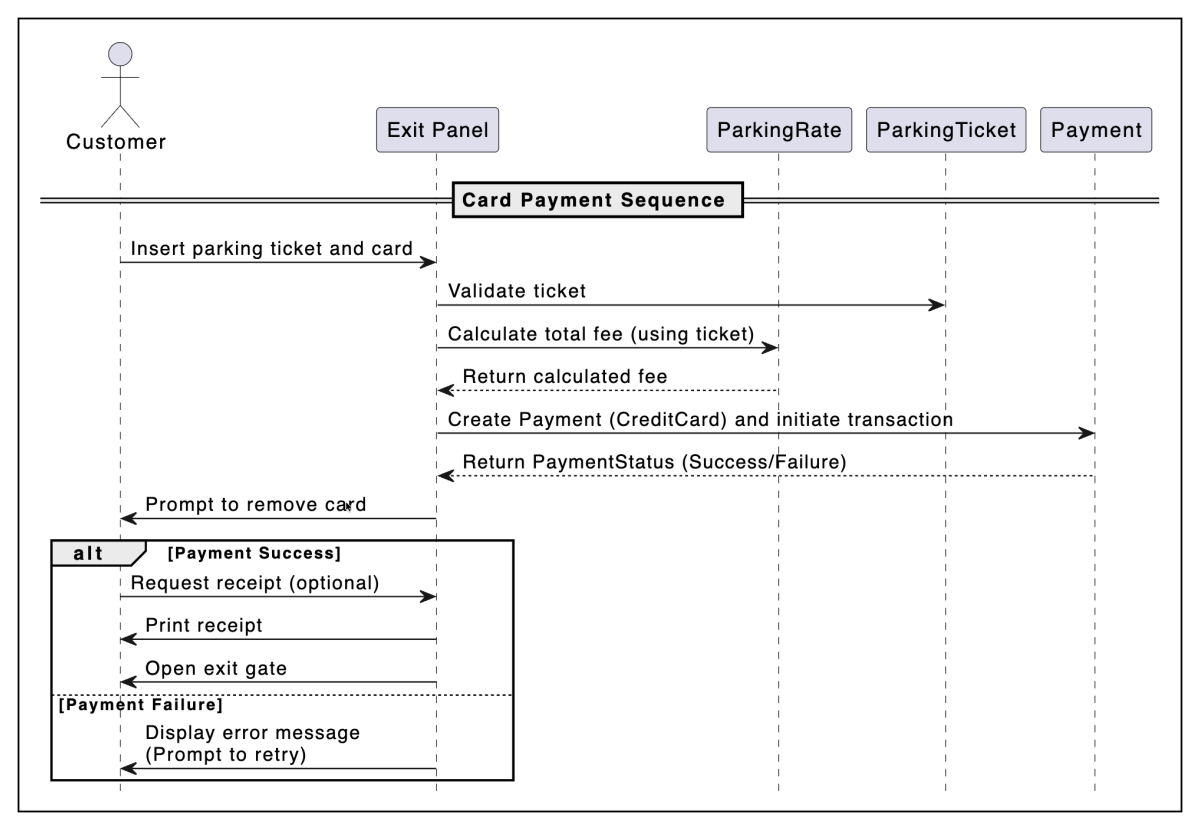
\includegraphics[width=0.5\textwidth]{Images/chapter_7/section_5942521041780736/5578538697490432.png}
 \caption{The sequence diagram for the card payment}
\end{figure}

\subsection{Sequence challenge: Payment verification}\label{fHxT_dVYp6FmPOr1CFhnN-1}
\\
In this section, you will help us complete a sequence diagram for the payment verification of a customer at the exit panel.
\\
The skeleton below represents the payment verification sequence diagram. Here , the ticket's payment status is currently unpaid, and the parking fee has to be calculated.

\begin{figure}[htbp]
 \centering
 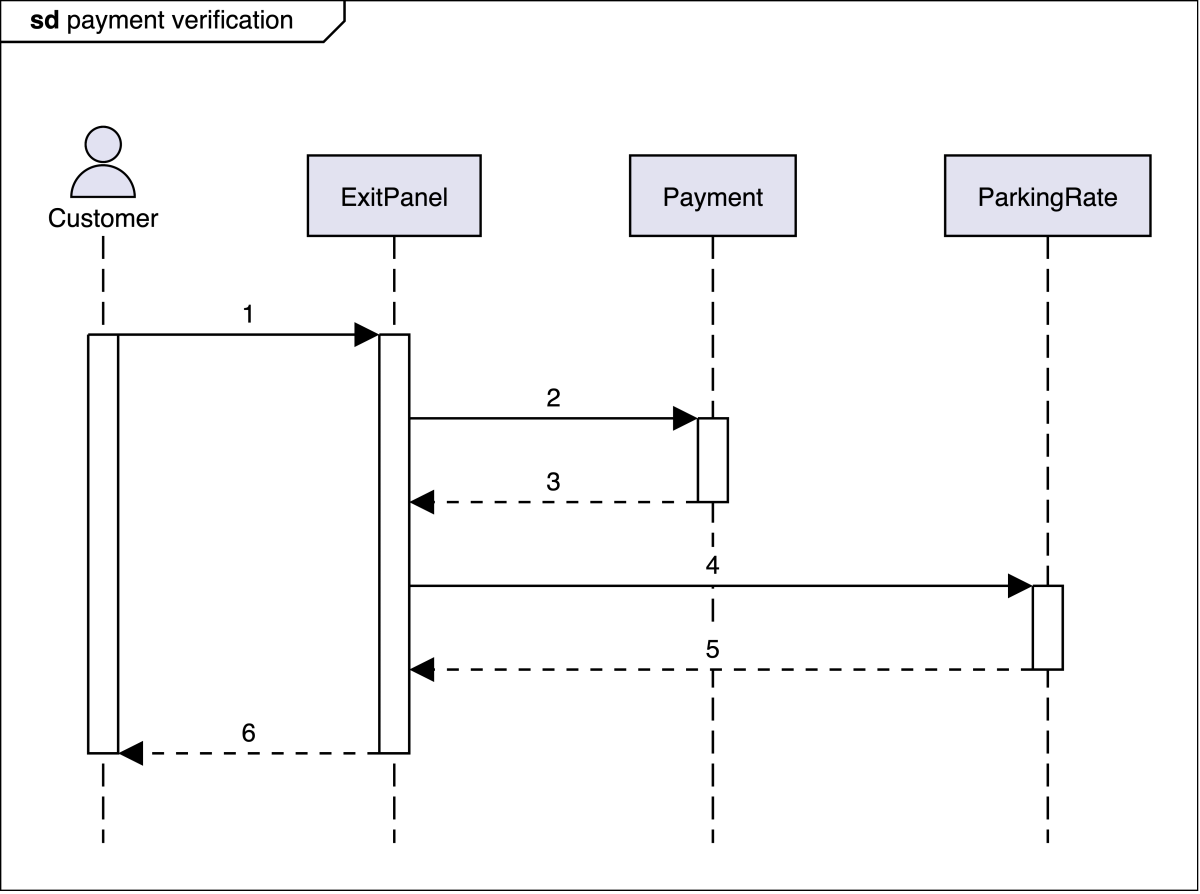
\includegraphics[width=0.5\textwidth]{Images/chapter_7/section_5942521041780736/5110471667744768.png}
 \caption{The sequence diagram for payment verification}
\end{figure}

Notice that the arrows in the diagram above are numbered from 1 to 6. The boxes below are the messages between the actor(s) and object(s). Can you rearrange the messages below in the correct order so that they appear in the skeleton of the sequence diagram above?
\begin{quote}
\textbf{Note:} If you're stuck, click the ``Show Solution'' button.
\end{quote}

Alternatively, you can also click the ``Show complete diagram'' button below to see the complete sequence diagram.

We will create activity diagrams for the parking lot design problem in the next lesson.

% End of section content